\documentclass[handout]{beamer}

\usepackage{Haust2017glærur}

\title{Tölvunarfræði 1a}
\subtitle{Vika 9, seinni fyrirlestur}

\begin{document}

\begin{frame}
\titlepage
\end{frame}

\section{Inngangur}

\begin{frame}{Í síðasta þætti\ldots}
    \begin{itemize}
    \item Innlestur skráa
    \begin{itemize}
        \item Línu fyrir línu
        \item Sem heild með \texttt{textscan}
    \end{itemize}
    \end{itemize}
\end{frame}

\subsection{Að skrifa í skrár}

\begin{frame}[fragile]{\texttt{fprintf} í skrá}
\begin{itemize}
 \item Aðalskipunin til að skrifa í skrár er \texttt{fprintf}
 \begin{itemize}
  \item Þetta er sama \texttt{fprintf} fall og við könnumst við
  \item Til að skrifa í skrána þarf að láta fallið fá skráarauðkenni sem fyrsta viðfang
 \end{itemize}
 \item Notkunin verður þá á borð við \verb|fprintf(fid, 'snið', breyta1, breyta2...)|
\end{itemize}
\end{frame}

\begin{frame}[fragile]{\texttt{fprintf} í skrá}
Dæmi:
\begin{minted}[frame=lines]{matlab}
fid = fopen('tilraun.txt', 'w');
for i = 1:5
    fprintf(fid, '%d: %d\n', i, randi(50));
end
fclose(fid);
\end{minted}
Ath. að hér er skráin \emph{yfirskrifuð} í hvert skipti. Til að skrifa aftast í skrá þarf að gefa \texttt{fopen} aðrar heimildir.
\end{frame}

\begin{frame}{Skráarheimildir}
\begin{center}
\begin{tabular}{ll}
\toprule
Regla&Lýsing\\
\midrule
\texttt{'r'}&Opnar skrá til lesturs\\
\texttt{'w'}&Opnar eða býr til skrá til skriftar, yfirskrifar\\
\texttt{'a'}&Opnar eða býr til skrá til skriftar, skrifar aftast\\
\texttt{'r+'}&Opnar skrá til skriftar eða lesturs\\
\texttt{'w+'}&Opnar eða býr til skrá til skriftar eða lesturs, yfirskrifar\\
\texttt{'a+'}&Opnar eða býr til skrá til skriftar eða lesturs, skrifar aftast\\
\bottomrule
\end{tabular}

\end{center}

\end{frame}

\section{Excel-skrár}

\begin{frame}{Excel-skrár}
\begin{itemize}
 \item Matlab getur unnið með Microsoft Excel skrár
 \begin{itemize}
  \item Viðkomandi föll: \texttt{xlswrite} og \texttt{xlsread}
 \end{itemize}
 \item Getur auðveldað flutning gagna á milli kerfa
\end{itemize}
\end{frame}

\begin{frame}[fragile]{\texttt{xlswrite}}
\begin{itemize}
 \item \texttt{xlswrite} skrifar fylki í Excel skrá
 \item Dæmi: Búum til $5 \times 3$ slembifylki og skrifum það í skrána \texttt{ranexcel.xls}
\begin{minted}[frame=lines]{matlab}
>> randomMatrix = randi(100, 5, 3); 
>> xlswrite('ranexcel.xls', randomMatrix); 
\end{minted}
\end{itemize}
\end{frame}

\begin{frame}[fragile]{\texttt{xlsread}}
\texttt{xlsread} les fylki úr Excel-skrá:

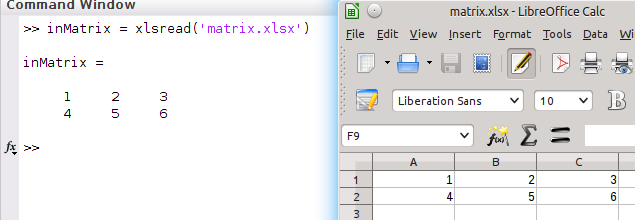
\includegraphics[width=\textwidth]{Pics/excel}

\end{frame}

\begin{frame}{Meira um Excel}
\begin{itemize}
 \item Excel-föllin hafa þó nokkra valkosti sem ekki er farið í hér
 \begin{itemize}
  \item Hægt er að lesa af mismunandi worksheets
  \item \texttt{help xlswrite} og \texttt{help xlsread}!
 \end{itemize}
 \item Til að fá fullan stuðning þarf að vera á Microsoft Windows stýrikerfi, með Microsoft Excel uppsett
 \begin{itemize}
  \item Grundvallarvirkni er þó alltaf til staðar
 \end{itemize}
\end{itemize}
\end{frame}

\section{Að vista breytur í .mat skrár}

\begin{frame}{Save og Load í nýjum buxum}
\begin{itemize}
 \item Hægt er að vista breytur vinnusvæðis í skrá með endinguna \texttt{.mat}
 \begin{itemize}
  \item \texttt{save} skipunin er notuð til að vista breytur í skrána
  \item \texttt{load} skipunin er notuð til að ná í þær aftur
 \end{itemize}
 \item Gagnlegt til að geyma vinnu tímabundið, t.d. til næsta vinnudags
 \item Galli: \texttt{.mat} skrár eru binary-skrár, önnur forrit en Matlab geta ekki lesið þær
\end{itemize}
\end{frame}

\begin{frame}[fragile]{Fyrirlestraræfing}
    \begin{columns}
    \column{0.7\textwidth}
    \begin{enumerate}
         \item Skrifið hitastigstöfluna til hægri í skrá, þannig að hver lína í skránni innihaldi lýsingu á borð við

         \texttt{Klukkan 0 var hitinn 12.5C}
         \item Skrifið hitastigstöfluna í Microsoft Excel skrá.
    \end{enumerate}
    \column{0.3\textwidth}
    \begin{center}
    \begin{tabular}{ll}
    \toprule
    Klst&$C^\circ$\\
    \midrule
    0&12.5\\
    3&12.4\\
    6&12.3\\
    9&12.8\\
    12&13.4\\
    15&14.0\\
    18&13.1\\
    21&12.8\\
    \bottomrule
    \end{tabular}
    \end{center}
    \end{columns}
\end{frame}

\begin{frame}{Viðbótardæmi}
    \begin{itemize}
        \item Dæmi 9.9
        \item Dæmi 9.12
        \item Dæmi 9.13
    \end{itemize}
\end{frame}

\end{document}
